


In this section we will explore the topoi-semantics for $\mathbb{FF}_2$/\emph{bushes} by following the general approach outlined in \cite{goldblatt}. 
\newline
We give, whenever necessary, a general outline from \cite{goldblatt} for topoi-semantics and make a few considerations with regards to $\mathbb{FF}_2$/\emph{bushes}.
 \newline\newline
Recall the sub-object classifier for  $\mathbb{FF}_2$/\emph{bushes}. 
\newline 
This is given by $\Omega= \{\textcolor{red}{\textbf{f}}, \textcolor{OliveGreen}{\textbf{t}} < \textcolor{cyan}{*}\}$ and $\mathbf{1} \xrightarrow{true} \Omega$. 
\newline
For each \emph{sub-object} $f : F \rightarrowtail G $ (which determines a sub-forest $f[F] \subseteq G$) there is a unique \emph{characteristic} arrow $\chi_f : F \rightarrow \Omega$ making the following commutative diagram a \emph{pullback} of $\chi_f$ and $true$.

\begin{figure}[h]
	\centering 
	\begin{tikzcd}
		F && G \\
		& {{}} \\
		1 && \Omega
		\arrow["s"', tail, from=1-1, to=1-3]
		\arrow["{\chi_f}"', from=1-3, to=3-3]
		\arrow["{!_F}", dashed, from=1-1, to=3-1]
		\arrow["true", from=3-1, to=3-3]
		\arrow[draw=none, from=1-1, to=2-2]
		\arrow[ from=1-1, to=2-2, phantom, "\scalebox{1.5}{$\lrcorner$}",  very near start, color=black]
	\end{tikzcd}\
	\caption{the characteristic diagram of $f$.}
\end{figure}   

Recall also that $\mathbb{Set}_{fin} \simeq \mathbb{FF}_1$. \newline
In $\mathbb{Set}_{fin}$ and more generally in $\mathbb{Set}$ the sub-object classifier is $\textbf{2} = \{0,1\} $ together with $\textbf{1}=\{0\} \xrightarrow{true} \textbf{2},\; 0 \mapsto 1$.\newline This can be translated in $\mathbb{FF}_1$ as \textbf{2} = \{\textcolor{red}{\textbf{f}}, \textcolor{OliveGreen}{\textbf{t}}\} with $\textbf{1}=\{\bullet\} \xrightarrow{true} \textbf{2}, \; \bullet \mapsto \textcolor{OliveGreen}{\textbf{t}}$.


\section{The Propositional Layer}
\label{chapter3}

Moving away from the usual environment of sets we wish to recover propositional Logic in the context of topoi.


\subsection{\hl{The Language of Topoi}}
 
\emph{	(Unless otherwise specified, the usual coloring notation to display maps is used. In the domain the fiber/pre-image of a node will have the same color of the node in the co-domain).} \newline

We begin the translation from the language of $\mathbb{Set}$ to that of a topos $\mathcal{E}$ from the truth constants $\top$,$\bot$ and the logical connectives $\neg,\land,\lor,\Rightarrow$. \newline
In all these cases they will be interpreted as arrows into $\Omega$ of the form $\Omega^n \rightarrow \Omega$, a.k.a. \emph{Truth-arrows} in which $n$ corresponds to the arity of the connective. \newline

Let's start by translating the constants true/top $\top$ and false/bottom $\bot$ in the context of our topos of \emph{bushes}.
\newline

Note that $\top$ has already been introduced as an arrow from the zero-th power of $\Omega$ to $\Omega$ i.e., $\textbf{1}= \Omega^0  \rightarrow \Omega$.
\newline In any topos $\mathcal{E}$, $\top$ is defined as $\textbf{1} \xrightarrow{true} \Omega$. In our case:
\begin{definition}[$\top$]
	$\top$ is $\textbf{1} \xrightarrow{true} \Omega$ the map $\bullet \mapsto \textcolor{OliveGreen}{\textbf{t}}$ .
\end{definition}

\begin{figure}[h]
	\centering
	\begin{tikzcd}
		{\textcolor{OliveGreen}{\bigcdot}} && 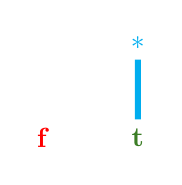
\begin{tikzpicture}[scale=0.4]
			\node (A) at (0,0) {\textcolor{red}{\textbf{f}}};
			\node (B) at (3,0) {\textcolor{OliveGreen}{\textbf{t}}};
			\node (C) at (3,3) {\textcolor{cyan}{$*$}};
			\draw[cyan, line width=.03in] (B) -- (C);
		\end{tikzpicture}
		\arrow["true", from=1-1, to=1-3]
	\end{tikzcd}
	\caption{$\top : \mathbf{1} \xrightarrow{true} \Omega$. (\emph{bushes})}
\end{figure}

This can also be seen as the \emph{characteristic arrow} for $\textbf{1} \xrightarrow{id} \textbf{1}$ i.e., for the \emph{maximal sub-object} of \textbf{1}. 
\newline
This generalizes from $\mathbb{Set}$ in which $\top : \textbf{1}=\{0\} \xrightarrow{true} \textbf{2}=\{0,1\}, \; 0 \mapsto 1$ is also the characteristic arrow for $\textbf{1} \xrightarrow{id} \textbf{1}$.

\newpage

In a similar vein, $\bot : \textbf{1}=\{0\} \xrightarrow{false} \textbf{2}=\{0,1\}, \; 0 \mapsto 0 $ in $\mathbb{Set}$ is the characteristic of $\emptyset \xrightarrow{\emptyset} \textbf{1}$ i.e., of the \emph{minimal sub-object} of \textbf{1}. 
\newline

It is straightforward to generalize this to an arbitrary topos $\mathcal{E}$ as the characteristic arrow $\bot$ of $0 \xrightarrow{!_0} 1$. In $\mathbb{FF}_2$ this becomes:

\begin{definition}[$\bot$]
	$\bot$ is $\textbf{1} \xrightarrow{false} \Omega$ the map $\bullet \mapsto \textcolor{red}{\textbf{f}}$.
\end{definition}

\begin{figure}[h]
	\centering
	\begin{tikzcd}
		{\textcolor{red}{\bigcdot}} && 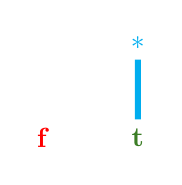
\begin{tikzpicture}[scale=0.4]
			\node (A) at (0,0) {\textcolor{red}{\textbf{f}}};
			\node (B) at (3,0) {\textcolor{OliveGreen}{\textbf{t}}};
			\node (C) at (3,3) {\textcolor{cyan}{$*$}};
			\draw[cyan, line width=.03in] (B) -- (C);
		\end{tikzpicture}
		\arrow["false", from=1-1, to=1-3]
	\end{tikzcd}
	\caption{$\bot : \mathbf{1} \xrightarrow{false} \Omega$. (\emph{bushes})}
\end{figure}

This is the characteristic arrow of the empty sub-forest $\textbf{0} \xrightarrow{0_1} \textbf{1}$.
\newline
Moving on to logical connectives.. 
\newpage

Starting with \emph{negation} $\neg$: This is a \emph{unary} operator and we expect a truth-arrow from $\Omega=\Omega^1 \rightarrow \Omega$. 
\newline
In $\mathbb{Set}$ $\textbf{2} \xrightarrow{\neg} \textbf{2}$ is the \emph{switch} function $\neg : 0 \mapsto 1, 1 \mapsto 0$. This coincides with the characteristic function of $\bot : \textbf{1}=\{0\} \xrightarrow{false} \textbf{2} = \{0,1\}$ which determines the sub-set $\{\bot(0)\}\subseteq \textbf{2}$. \newline
In the language of topoi: $\neg$ is the characteristic arrow of $\bot$ as defined previously. So:

\begin{definition}[$\neg$]
	$\neg : \Omega \rightarrow \Omega$ is the characteristic arrow of $\bot : \textbf{1} \xrightarrow{false} \Omega$.
\end{definition}

This means that the following commutative diagram is a pullback in $\mathbb{FF}_2$.

\begin{figure}[h]
	\centering 
	\begin{tikzcd}
		\begin{tikzpicture}[scale=0.4]
		\node (A) at (0,0) {\textcolor{black}{$\bigcdot$}};
	\end{tikzpicture} &&  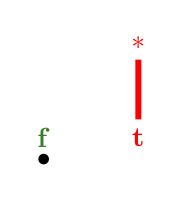
\begin{tikzpicture}[scale=0.4]
			\node (A) at (0,0) {\textcolor{OliveGreen}{\textbf{f}}};
			\node (A') at (0,-0.7) {$\bullet$};
			\node (B) at (3,0) {\textcolor{red}{\textbf{t}}};
			\node (C) at (3,3) {\textcolor{red}{$*$}};
			\draw[red, line width=.03in] (B) -- (C);
		\end{tikzpicture} \\
		& {{}} \\
		\begin{tikzpicture}[scale=0.4]
			\node (A) at (0,0) {\textcolor{OliveGreen}{$\bigcdot$}};
			\node (A') at (0,-0.7) {\textcolor{black}{$\bullet$}};	
	\end{tikzpicture} && 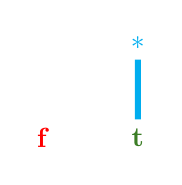
\begin{tikzpicture}[scale=0.4]
		\node (A) at (0,0) {\textcolor{red}{\textbf{f}}};
		\node (B) at (3,0) {\textcolor{OliveGreen}{\textbf{t}}};
		\node (C) at (3,3) {\textcolor{cyan}{$*$}};
		\draw[cyan, line width=.03in] (B) -- (C);
	\end{tikzpicture}
		\arrow["\bot"', tail, from=1-1, to=1-3]
		\arrow["{\neg}"', from=1-3, to=3-3]
		\arrow["{!_1}", dashed, from=1-1, to=3-1]
		\arrow["true", from=3-1, to=3-3]
		\arrow[draw=none, from=1-1, to=2-2]
		\arrow[ from=1-1, to=2-2, phantom, "\scalebox{1.5}{$\lrcorner$}",  very near start, color=black]
	\end{tikzcd}\
	\caption{the characteristic diagram of $\bot$. The images of \textbf{1} by $\bot$ and $!_1$ are shown with a black bullet underneath. }
\end{figure}   
\newpage
In the case of \emph{conjunction} $\land$, as a binary operator we expect a truth arrow $\Omega \times \Omega = \Omega^2 \rightarrow \Omega$. 
\newline
For $\mathbb{Set}$ $\land$ is the characteristic function of $\{ (1,1) \} \subset \textbf{2}\times\textbf{2}$ since by the correspondence $0 \leftrightarrow $ \textcolor{red}{\textbf{f}} and $1 \leftrightarrow $ \textcolor{OliveGreen}{\textbf{t}}, $\land$ classically outputs \textcolor{OliveGreen}{\textbf{t}} only on the pair (\textcolor{OliveGreen}{\textbf{t}},\textcolor{OliveGreen}{\textbf{t}}). As an arrow in $\mathbb{Set}$ this sub-set is determined by the \emph{product-function} $\top \times \top : \textbf{1} \times \textbf{1} \rightarrow \textbf{2} \times \textbf{2}$. \newline
We can define $\land$ in any topos as the character of the product arrow $\top \times \top$.\newline
In \emph{bushes}:

\begin{definition}[$\land$]
	$\land$ is the characteristic arrow of $\top \times \top : \textbf{1} \times \textbf{1} \rightarrow \Omega \times \Omega$.
\end{definition}

Recalling that  $ \Omega \times \Omega = (\textbf{1} + \textbf{1}_\bot) \times (\textbf{1} + \textbf{1}_\bot) = \textbf{1} + \textbf{1}_\bot + \textbf{1}_\bot + (\textbf{1}_\bot \times \textbf{1}_\bot)   $ and $\textbf{1} \times \textbf{1} = \textbf{1} $
the characteristic diagram is the following:

\begin{figure}[h]
	\centering 
	\begin{tikzcd}
		\begin{tikzpicture}[scale=0.4]
			\node (A) at (0,0) {\textcolor{black}{$\bigcdot$}};
		\end{tikzpicture} && 
\begin{tikzpicture}[scale=0.4]
		\node (A) at (0,0) {\textcolor{red}{$\bigcdot$}};
		\node (B) at (2,0) {\textcolor{red}{$\bigcdot$}};
			\node (C) at (2,3) {\textcolor{red}{$\bigcdot$}};
		\node (D) at (4,0) {\textcolor{red}{$\bigcdot$}};
			\node (E) at (4,3) {\textcolor{red}{$\bigcdot$}};
		\node (F) at (8,0) {\textcolor{OliveGreen}{$\bigcdot$}};
		\node (F') at (8,-0.7) {\textcolor{black}{$\bullet$}};	
			\node (G) at (6,3) {\textcolor{cyan}{$\bigcdot$}};
			\node (H) at (8,3) {\textcolor{cyan}{$\bigcdot$}};
			\node (I) at (10,3) {\textcolor{cyan}{$\bigcdot$}};
		\draw[red, line width=.03in] (B) -- (C);
		\draw[red, line width=.03in] (D) -- (E);
		\draw[cyan, line width=.03in] (F) -- (G);
		\draw[cyan, line width=.03in] (F) -- (H);
		\draw[cyan, line width=.03in] (F) -- (I);	
\end{tikzpicture} \\
		& {{}} \\
		\begin{tikzpicture}[scale=0.45]
			\node (A) at (0,0) {\textcolor{OliveGreen}{$\bigcdot$}};
			\node (A') at (0,-0.7) {\textcolor{black}{$\bullet$}};	
		\end{tikzpicture} && 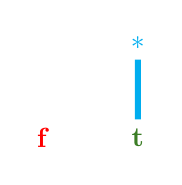
\begin{tikzpicture}[scale=0.4]
			\node (A) at (0,0) {\textcolor{red}{\textbf{f}}};
			\node (B) at (3,0) {\textcolor{OliveGreen}{\textbf{t}}};
			\node (C) at (3,3) {\textcolor{cyan}{$*$}};
			\draw[cyan, line width=.03in] (B) -- (C);
		\end{tikzpicture}
		\arrow["\top \times \top"', tail, from=1-1, to=1-3]
		\arrow["{\land}"', from=1-3, to=3-3]
		\arrow["{!_{1 \times 1}}", dashed, from=1-1, to=3-1]
		\arrow["true", from=3-1, to=3-3]
		\arrow[draw=none, from=1-1, to=2-2]
		\arrow[ from=1-1, to=2-2, phantom, "\scalebox{1.5}{$\lrcorner$}",  very near start, color=black]
	\end{tikzcd}\
	\caption{the characteristic diagram of $\top \times \top$.  }
\end{figure}   

\newpage
The case of $\lor$ is analogous to $\land$: \newline
Starting as usual from $\mathbb{Set}$, $\lor$ is the characteristic function of the sub-set $D = \{(1,1),(0,1)\} \cup \{(1,1),(1,0)\}=\{(0,1),(1,0),(1,1)\} \subset \textbf{2}\times\textbf{2}$. The two sub-sets $\{(1,1),(0,1)\}$ and $\{(1,1),(1,0)\}$ are determined by the arrows $id_2 \times \top, \top \times id_2 : \textbf{2} \rightarrow \textbf{2} \times \textbf{2}$ so their union $D$ is the image of the \emph{sum-function} $(id_2 \times \top) + (\top \times id_2) : \textbf{2} + \textbf{2} \rightarrow \textbf{2} \times \textbf{2} $. \newline
As such we can define $\lor$ in any topos as the character of the image of the \emph{coproduct-arrow} $f = (id_\Omega \times \top) + (\top \times id_\Omega)$ i.e., the characteristic arrow of $Im(f) \xrightarrow{m} \Omega \times \Omega$ \footnote{obtained through epi-mono factorization $f=m \circ e$.}.
In \emph{bushes}:

\begin{definition}[$\lor$] 
$\lor$ is the character of the image of  $(id_\Omega \times \top) + (\top \times id_\Omega) : \Omega + \Omega \rightarrow \Omega \times \Omega $.
\end{definition}


\begin{figure}[h]
	\centering
	\begin{tikzcd}
		\begin{tikzpicture}[scale=0.4]
			\node (A) at (0,0) {\textcolor{purple}{$\bigcdot$}};
			\node (B) at (2,0) {\textcolor{YellowGreen}{$\bigcdot$}};
			\node (C) at (2,3) {\textcolor{blue}{$\bigcdot$}};
			\node (D) at (4,0) {\textcolor{orange}{$\bigcdot$}};
			\node (E) at (6,0) {\textcolor{green}{$\bigcdot$}};
			\node (F) at (6,3) {\textcolor{CadetBlue}{$\bigcdot$}};
			\draw[blue, line width=.01in] (B) -- (C);	
			\draw[CadetBlue, line width=.01in] (E) -- (F);	
		\end{tikzpicture} \\
		\\
		\begin{tikzpicture}[scale=0.4]
			
			\node (B) at (2,0) {\textcolor{black}{$\bigcdot$}};
			\node (b) at (2,-0.7) {\textcolor{purple}{$\bullet$}};
			\node (D) at (4,0) {\textcolor{black}{$\bigcdot$}};
			\node (d) at (4,-0.7) {\textcolor{orange}{$\bullet$}};
			\node (F) at (8,0) {\textcolor{black}{$\bigcdot$}};
			\node (f) at (7.8,-0.7) {\textcolor{YellowGreen}{$\bullet$}};	
			\node (f') at (8.3,-0.7) {\textcolor{green}{$\bullet$}};
			\node (G) at (6,3) {\textcolor{black}{$\bigcdot$}};
			\node (g) at (6,2.3) {\textcolor{blue}{$\bullet$}};
			\node (I) at (10,3) {\textcolor{black}{$\bigcdot$}};
			\node (i) at (10,2.3) {\textcolor{CadetBlue}{$\bullet$}};

			\draw[line width=.01in] (F) -- (G);
			\draw[line width=.01in] (F) -- (I);	
		\end{tikzpicture} && 
\begin{tikzpicture}[scale=0.4]
			\node (A) at (0,0) {\textcolor{red}{$\bigcdot$}};
			\node (B) at (2,0) {\textcolor{OliveGreen}{$\bigcdot$}};
			\node (b) at (2,-0.7) {\textcolor{purple}{$\bullet$}};
			\node (C) at (2,3) {\textcolor{cyan}{$\bigcdot$}};
			\node (D) at (4,0) {\textcolor{OliveGreen}{$\bigcdot$}};
			\node (d) at (4,-0.7) {\textcolor{orange}{$\bullet$}};
			\node (E) at (4,3) {\textcolor{cyan}{$\bigcdot$}};
			\node (F) at (8,0) {\textcolor{OliveGreen}{$\bigcdot$}};
			\node (f) at (7.8,-0.7) {\textcolor{YellowGreen}{$\bullet$}};	
			\node (f') at (8.3,-0.7) {\textcolor{green}{$\bullet$}};
			\node (G) at (6,3) {\textcolor{OliveGreen}{$\bigcdot$}};
			\node (g) at (6,2.3) {\textcolor{blue}{$\bullet$}};
			\node (H) at (8,3) {\textcolor{cyan}{$\bigcdot$}};
			\node (I) at (10,3) {\textcolor{OliveGreen}{$\bigcdot$}};
			\node (i) at (10,2.3) {\textcolor{CadetBlue}{$\bullet$}};
			\draw[cyan, line width=.03in] (B) -- (C);
			\draw[cyan, line width=.03in] (D) -- (E);
			\draw[OliveGreen, line width=.03in] (F) -- (G);
			\draw[cyan, line width=.03in] (F) -- (H);
			\draw[OliveGreen, line width=.03in] (F) -- (I);	
		\end{tikzpicture} \\
		\\
			\begin{tikzpicture}[scale=0.45]
			\node (A) at (0,0) {\textcolor{OliveGreen}{$\bigcdot$}};
		
		\end{tikzpicture} && 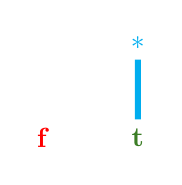
\begin{tikzpicture}[scale=0.4]
		\node (A) at (0,0) {\textcolor{red}{\textbf{f}}};
		\node (B) at (3,0) {\textcolor{OliveGreen}{\textbf{t}}};
		\node (C) at (3,3) {\textcolor{cyan}{$*$}};
		\draw[cyan, line width=.03in] (B) -- (C);
	\end{tikzpicture}
		\arrow["true", from=5-1, to=5-3]
		\arrow["{!_{Im (f)}}", from=3-1, to=5-1]
		\arrow[tail, "m", from=3-1, to=3-3]
		\arrow["{\lor}", from=3-3, to=5-3]
		\arrow["{(id_\Omega \times \top) + (\top \times id_\Omega)}", from=1-1, to=3-3]
		\arrow[two heads,"e"', from=1-1, to=3-1]
		\arrow[draw=none, from=3-1, to=5-3]
		\arrow[ from=3-1, to=5-3, phantom, "\scalebox{1.5}{$\lrcorner$}",  very near start, color=black]
	\end{tikzcd}

\caption{the characteristic diagram of $Im((id_\Omega \times \top) + (\top \times id_\Omega))$ with the epi-mono factorization on display. \newline
	The images of the nodes $\Omega + \Omega$ are shown with bullets of matching color.  }
\end{figure}


\newpage
Finally we arrive at implication $\Rightarrow$. \newline
Starting from $\mathbb{Set}$ we observe that the sub-set that we want to \emph{characterize} for implication is precisely $\leq \;= \{(0,0), (0,1), (1,1)\} \subset \textbf{2} \times \textbf{2}$ i.e., the partial order relation on the \emph{lattice} \textbf{2} given by $\leq \;= \{(x,y) \in \textbf{2} \times \textbf{2} : x \leq y\}$. $\leq$ can also be described as $\leq \;= \{(x,y) \in \textbf{2} \times \textbf{2} : x \land y = x\}$ i.e., the \emph{equalizer}  of $\land$ and $\pi_1$ the first projection of $\textbf{2} \times \textbf{2}$ denoted by $Eq(\land,\pi_1) = \;\leq \;\overset{e}{\rightarrowtail} \textbf{2} \times \textbf{2}\; \substack{\xrightarrow[\pi_1]{}\\[-2.2em] \xrightarrow[]{\land\;}} \; \textbf{2}$. \newline
This allows us to state that in any topos: \newline $\Rightarrow$ is the character of the equalizer $e$ of $\land$ as previously defined and $\pi_1$ the first projection of $\Omega \times \Omega$. As such in \emph{bushes}:

\begin{definition}[$\Rightarrow$] 
$\Rightarrow$ is the character of $e$ with $Eq(\land,\pi_1) = E \overset{e}{\rightarrowtail} \Omega \times \Omega\; \substack{\xrightarrow[\pi_1]{}\\[-2.2em] \xrightarrow[]{\land\;}} \; \Omega$.
\end{definition}
The characteristic diagram is thus given by:

\begin{figure}[h]
	\centering 
	\begin{tikzcd}
		\begin{tikzpicture}[scale=0.4]
			\node (A) at (0,0) {\textcolor{orange}{$\bigcdot$}};
			\node (B) at (2,0) {\textcolor{GreenYellow}{$\bigcdot$}};
			\node (C) at (2,3) {\textcolor{blue}{$\bigcdot$}};
			\node (F) at (8,0) {\textcolor{green}{$\bigcdot$}};
			\node (G) at (6,3) {\textcolor{CadetBlue}{$\bigcdot$}};
			\node (H) at (8,3) {\textcolor{RoyalBlue}{$\bigcdot$}};
			\draw[blue, line width=.01in] (B) -- (C);
			\draw[CadetBlue, line width=.01in] (F) -- (G);
			\draw[RoyalBlue, line width=.01in] (F) -- (H);
		\end{tikzpicture} && 
\begin{tikzpicture}[scale=0.4]
			\node (A) at (0,0) {\textcolor{OliveGreen}{$\bigcdot$}};
			\node (a) at (0,-0.7) {\textcolor{orange}{$\bullet$}};
			\node (B) at (2,0) {\textcolor{OliveGreen}{$\bigcdot$}};
			\node (b) at (2,-0.7) {\textcolor{GreenYellow}{$\bullet$}};
			\node (C) at (2,3) {\textcolor{OliveGreen}{$\bigcdot$}};
			\node (c) at (2,2.3) {\textcolor{blue}{$\bullet$}};
			\node (D) at (4,0) {\textcolor{red}{$\bigcdot$}};
			\node (E) at (4,3) {\textcolor{red}{$\bigcdot$}};
			\node (F) at (8,0) {\textcolor{OliveGreen}{$\bigcdot$}};
			\node (f) at (8,-0.7) {\textcolor{green}{$\bullet$}};	
			\node (G) at (6,3) {\textcolor{OliveGreen}{$\bigcdot$}};
			\node (g) at (6,2.3) {\textcolor{CadetBlue}{$\bullet$}};
			\node (H) at (8,3) {\textcolor{OliveGreen}{$\bigcdot$}};
			\node (h) at (8,2.3) {\textcolor{RoyalBlue}{$\bullet$}};
			\node (I) at (10,3) {\textcolor{cyan}{$\bigcdot$}};
			\draw[OliveGreen, line width=.03in] (B) -- (C);
			\draw[red, line width=.03in] (D) -- (E);
			\draw[OliveGreen, line width=.03in] (F) -- (G);
			\draw[OliveGreen, line width=.03in] (F) -- (H);
			\draw[cyan, line width=.03in] (F) -- (I);	
		\end{tikzpicture} \\
		& {{}} \\
		\begin{tikzpicture}[scale=0.45]
			\node (A) at (0,0) {\textcolor{OliveGreen}{$\bigcdot$}};
		\end{tikzpicture} && 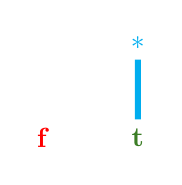
\begin{tikzpicture}[scale=0.4]
			\node (A) at (0,0) {\textcolor{red}{\textbf{f}}};
			\node (B) at (3,0) {\textcolor{OliveGreen}{\textbf{t}}};
			\node (C) at (3,3) {\textcolor{cyan}{$*$}};
			\draw[cyan, line width=.03in] (B) -- (C);
		\end{tikzpicture}
		\arrow["e", tail, from=1-1, to=1-3]
		\arrow["{\Rightarrow}"', from=1-3, to=3-3]
		\arrow["{!_E}", dashed, from=1-1, to=3-1]
		\arrow["true", from=3-1, to=3-3]
		\arrow[draw=none, from=1-1, to=2-2]
		\arrow[ from=1-1, to=2-2, phantom, "\scalebox{1.5}{$\lrcorner$}",  very near start, color=black]
	\end{tikzcd}\
	\caption{the characteristic diagram of $e$. \newline
		The images of the nodes of $E$ are shown with bullets of matching color.  }
\end{figure}  

\newpage
We give some general notions from \cite{goldblatt}: \newline
\newline
Let's consider a generic topos $\mathcal{E}$. \newline
We defined the \emph{truth-arrows} we need for the semantics of propositional formulae.  \newline
The \emph{truth-values} are given by the \emph{hom-set} $\mathcal{E}(\textbf{1},\Omega)$. \newline Note that these truth-values are in fact \emph{generalized elements} of $\Omega$ which generalize the set-elements of $\mathbf{2}$ in $\mathbb{Set}$. \newline
An \emph{$\mathcal{E}-valuation$} of a propositional variable is just an assignment of a truth-value. This can be extended inductively to formulae using the connectives we just defined:

\begin{definition}[$\mathcal{E}$ -valuation]
	An \emph{$\mathcal{E}$-valuation} is a function $V : \mathbf{Prop} \rightarrow \mathcal{E}(\mathbf{1},\Omega)$ which is extended to $\mathbf{Form}$: \newline
	  $\forall \phi,\psi \in \mathbf{Form}$ :
	\begin{itemize}
		\item $V(\neg \phi) = \neg \circ V(\phi)$.
		\item $V(\phi \land \psi) =\; \land \circ  [V(\phi)\times V(\chi)] $.
		\item $V(\phi \lor \psi) =\; \lor \circ  [V(\phi)\times V(\chi)] $.
		\item $V(\phi \Rightarrow \psi) =\; \Rightarrow \circ  [V(\phi)\times V(\chi)] $.
	\end{itemize}
\end{definition}

We can talk about \emph{topos-validity} of a formula $\phi$ if every valuation gives the truth-arrow $\top$:

\begin{definition}[$\mathcal{E}$-validity (propositional)]
	A formula $\phi$ is $\mathcal{E}$-valid, denoted by $\mathcal{E} \models \phi$ or $\models_\mathcal{E}  \phi$, when for every $\mathcal{E}$-valuation $V$, $V(\phi)=\top$.  
\end{definition} 




\newpage
\subsection{The Algebra of Sub-Objects}

Let $\mathcal{E}$ be a topos and $\textbf{d}\in \mathcal{E}$ one of its objects. \newline
The truth arrows defined previously can be used to give an algebraic structure to $Sub(\textbf{d})$ the collection of sub-objects of $\textbf{d}$. \newline
In the case of $\mathbb{Set}$, consider sub-objects or simply sub-sets $A$ and $B$ of a set $D$ with their characteristic functions $\chi_A, chi_B : D \rightarrow \textbf{2} $ then we have the following:
\begin{itemize}
	\item $\chi_{A^c} = \neg \circ \chi_A$.
	\item $\chi_{A \cap B} = \land \circ (\chi_A \times \chi_B)$.
	\item $\chi_{A \cup B} = \lor \circ (\chi_A \times \chi_B)$.	
\end{itemize}  

Generalizing to $\mathcal{E}$:
\newline

We define the operations in $Sub(\textbf{d})$ by specifying the \emph{characteristic arrow} $\chi : \textbf{d} \rightarrow \Omega$ of the new sub-object which will then be obtained via the pullback of $\top$ and $\chi$. \newline
Let $f,g \in Sub(d)$ we define the complement of $f$ as:

\begin{definition}[$-f$]
	The complement of $f$ is the sub-object $-f$ whose characteristic arrow is $\neg \circ \chi_f$.  
\end{definition}

The intersection of $f$ and $g$ as:

\begin{definition}[$f \cap g$]
	The intersection of $f$ and $g$ is the sub-object $f \cap g$ whose characteristic arrow is $\land \circ (\chi_f \times \chi_g)$.	
\end{definition}

The union of $f$ and $g$ as:

\begin{definition}[$f \cup g$]
	The union of $f$ and $g$ is the sub-object $f \cup g$ whose characteristic arrow is $\lor \circ (\chi_f \times \chi_g)$.	
\end{definition}

The implication of $g$ by $f$ as:

\begin{definition}[$f \Rightarrow g$]
	The implication of $g$ by $f$ is the sub-object $f \Rightarrow g$ whose characteristic arrow is $\Rightarrow \circ (\chi_f \times \chi_g)$.	
\end{definition}

Recall that just like ($\mathcal{P}(D), \leq$) is a partial ordering with set-inclusion, $(Sub(d), \sqsubseteq)$
becomes a partial ordering by \emph{sub-object inclusion} i.e., $f \sqsubseteq g$ if there is an arrow $h: Dom(f) \rightarrow Dom(g)$ such that $f = g \circ h$.\newline
We now have the following result:

\begin{prop}
	$(Sub(d),\sqsubseteq)$ is a \emph{bounded lattice} in which:
	\begin{itemize}
		\item $f \cap g$ is the \emph{greatest lower bound} of $f$ and $g$ i.e., the \emph{meet} of $f$ and $g$.
		\item $f \cup g$ is the \emph{least upper bound} of $f$ and $g$ i.e., the \emph{join} of $f$ and $g$.
		\item the arrow from the initial object $0_d : \textbf{0} \rightarrow \textbf{d}$ is the \emph{bottom} element.
		 \item the identity arrow $1_d : \textbf{d} \rightarrow \textbf{d}$ is the \emph{top} element.
	\end{itemize}
\end{prop}

Also the following holds for all $f,g,h \in Sub(\textbf{d})$ making $\Rightarrow$ a \emph{pseudo-complement}:

\begin{lem}
	$h \sqsubseteq (f \Rightarrow g) $ iff $ (f \cap h) \sqsubseteq g $.
\end{lem}

We are thus in a position to state that:

\begin{thm}
	$(Sub(d),\sqsubseteq)$ is a \emph{Heyting Algebra} with top element $1_d$, bottom element $0_d$ and $f\cap g$,$f \cup g$ and $f \Rightarrow g$ are respectively the \emph{meet}, \emph{join} and \emph{pseudo-complement} operations.
\end{thm}

We also have:

\begin{thm}
	$(\mathcal{E}(\textbf{d},\Omega), \sqsubseteq)$ is a \emph{Heyting Algebra} with top element $true_d$ \footnote{the character of $1_d$ i.e., the identity arrow on $d$. }, bottom element $false_d$ \footnote{the character of $0_d: 0 \rightarrow d$ i.e., the initial arrow on $d$.} and the truth-arrows as operations.
	This can be seen by the following definitions:
	\begin{gather*}
		\chi_f \sqsubseteq \chi_g \text{ iff }(\chi_f \times \chi_g)\text{ factors through }e: \leq \hookrightarrow \Omega \times \Omega. \\
		\chi_f \cap \chi_g :=\;\; \land \circ (\chi_f \times \chi_g). \\
		\chi_f \cup \chi_g :=\;\; \lor \circ (\chi_f \times \chi_g). \\
		\neg\chi_f :=\;\; \neg \circ \chi_f. \\
		\chi_f \Rightarrow \chi_g :=\;\; \Rightarrow \circ (\chi_f \times \chi_g). \\
	\end{gather*}
\end{thm} 
\newpage
Recall that the $\Omega$-Axiom from \ref{chapter02} gave us a bijection $Sub(d) \cong \mathcal{E}(\textbf{d},\Omega)$ in which $f \xleftrightarrow{1:1} \chi_f$.\newline
We can show that this bijection is in fact a \emph{Heyting Algebra isomorphism} $\Delta: Sub(d) \cong \mathcal{E}(\textbf{d},\Omega)$ where: 
\begin{gather*}
	\Delta(-f) :=\;\; \neg \circ \Delta(f). \\
	\Delta(f \cap g) :=\;\; \land \circ (\Delta(f) \times \Delta(g)). \\
	\Delta(f \cup g) :=\;\; \lor \circ (\Delta(f) \times \Delta(g)). \\
	\Delta(f \Rightarrow g) =\;\; \Rightarrow \circ (\Delta(f) \times \Delta(g)). 
\end{gather*}


\newpage
\subsection{Soundness and Completeness for CPL and IPL}

We proceed by giving a few more general results from \cite{goldblatt}:\newline

We have seen that in any topos $\mathcal{E}$ the truth arrow $\top = \chi_{id_\textbf{1}}$ and $\bot = \chi_{0_\textbf{1}}$. \newline
If we now focus on the sub-objects of the terminal \textbf{1} i.e., $Sub(\textbf{1})$  we can derive the following: 
\begin{itemize}
	\item $\top \land \top = \chi_{id_\textbf{1}} \land \chi_{id_\textbf{1}} = \chi_{id_\textbf{1} \cap id_\textbf{1}}$ = $\chi_{id_\textbf{1}} = \top$. 
	\item $\top \land \bot = \chi_{id_\textbf{1}} \land \chi_{0_\textbf{1}} = \chi_{id_\textbf{1} \cap 0_\textbf{1}}$ = $\chi_{0_\textbf{1}} = \bot$.
	\item $\bot \land \top = \chi_{0_\textbf{1}} \land \chi_{id_\textbf{1}} = \chi_{0_\textbf{1} \cap id_\textbf{1}}$ = $\chi_{0_\textbf{1}} = \bot$.
	 \item $\bot \land \bot = \chi_{0_\textbf{1}} \land \chi_{0_\textbf{1}} = \chi_{0_\textbf{1} \cap 0_\textbf{1}}$ = $\chi_{0_\textbf{1}}  = \bot$.
	\item ... 	 
\end{itemize}
and so forth for $\lor$ and $\Rightarrow$.
What we found is that the truth arrows $\top$ and $\bot$ behave \emph{classically} with respect to the $\mathcal{E}$-connectives we defined. \footnote{the same result could have been obtained without reference to sub-objects and simply unfolding the definitions, putting one pullback square atop another.} 

With this in mind and remembering how we defined $\mathcal{E}$-validity, we can give some first results about Soundness and Completeness for \emph{Classical} and \emph{Intuitionistic} Propositional Logic \textbf{CPL} and \textbf{IPL}. \newline

Namely, \emph{Completeness} for \textbf{CPL}: 

\begin{thm}
	For any topos $\mathcal{E}$, $\alpha \in \mathbf{Form}$:
	\begin{equation*}
		\text{If }\mathcal{E} \models \alpha\text{ then }\vdash_{CPL} \alpha.
	\end{equation*} 
\end{thm}

\textbf{CPL} is not always \emph{sound} with respect $\mathcal{E}$-validity.. \newline
However, if we restrict ourselves to \emph{bivalent} topoi i.e., topoi with just two truth values i.e., $|\mathcal{E}(\textbf{1}, \Omega)|=2$ we have soundness and completeness for \textbf{CPL}:
\begin{prop}\label{bivalence}
	If $\mathcal{E}$ is bivalent, then:
	\begin{gather*}
		\forall \alpha \in \textbf{Form}:\\ 
		\mathcal{E} \models \alpha \text{ iff } \vdash_{CPL} \alpha.
	\end{gather*}
	
	For example:\newline
	$\mathbb{Set}$ is bivalent as $\Omega = \mathbb{2} = \{0,1\}$ and thus:
	\begin{equation*}
		\vdash_{CPL} \alpha \; \text{ iff } \; \mathbb{Set} \models \alpha.
	\end{equation*}
\end{prop}

What about \emph{intuitionistic} Logic? \newline

Recall that Heyting Algebras provide a sound and complete semantics for \textbf{IPL} i.e.,:

\begin{remark}
	For any Heyting Algebra \emph{HA}, $\alpha \in \mathbf{Form}$:
	\begin{equation*}
		\emph{HA} \models \alpha\text{ iff }\vdash_{IPL} \alpha.
	\end{equation*}
	 
\end{remark}

As we have seen, for any $\mathcal{E}$-object $\mathbf{d}$, there is an isomorphism $Sub(d) \cong \mathcal{E}(\textbf{d},\Omega)$ which transfers the H.A. \footnote{from now on H.A. will be more commonly used instead of \emph{Heyting Algebra}. } structure of the sub-objects of $Sub(d)$ to the truth arrows of $\mathcal{E}(\textbf{d},\Omega)$. \newline
 This gives us the following equivalence which links the semantics of topoi to that of Heyting Algebras:\newline
($\models_{\mathcal{E}}$ denotes topos validity whilst $\models_{H.A.}$ Heyting algebra validity).
\begin{prop}
	For any topos $\mathcal{E}$, $\alpha \in \mathbf{Form}$:
	\begin{equation*}
		\models_\mathcal{E} \alpha\text{ iff }\;\;\mathcal{E}(\textbf{1},\Omega) \models_{H.A.} \alpha\text{ iff }\;\;Sub(\textbf{1}) \models_{H.A.} \alpha.
	\end{equation*}
\end{prop}
To see why this is the case, notice that an $\mathcal{E}$-valuation is an H.A.-valuation for $\mathcal{E}(\textbf{1},\Omega)$ which is isomorphic to $Sub(\textbf{1})$ and that the \emph{unit} $\top$ of the H.A. $\mathcal{E}(\textbf{1},\Omega)$ is precisely the truth arrow $\top : \textbf{1}\rightarrow \Omega$ so that $\mathcal{E}$-validity and $\mathcal{E}(\textbf{1},\Omega)$-validity amount to the same thing. 


This allows us to say that if $\vdash_{IPL} \alpha$, then by soundness for Heyting Algebras $Sub(\textbf{1})\models \alpha$ and $\mathcal{E}(\textbf{1}, \Omega) \models \alpha$ which means $\models_\mathcal{E}  \alpha$. \newline
What we have shown is, contrary to the case of \textbf{CPL}, that topoi provide a sound semantics for \textbf{IPL}.

\begin{thm}[Soundness for topos-validity]
		For any topos $\mathcal{E}$, $\alpha \in \mathbf{Form}$:
		\begin{equation*}
			\text{If }\vdash_{IPL} \alpha\text{ then }\models_\mathcal{E}  \alpha.
		\end{equation*}		
\end{thm}


\newpage
\subsection{\hl{External and Internal Logics}}
\label{externalandint}

Let's take a step back and revisit our definitions for the logical connectives in the topos of \emph{bushes}/$\mathbb{FF_2}$. 
\newline
Negation $\neg$ for example yielded:
\begin{figure}[h]
	\centering
	\begin{tikzcd}
		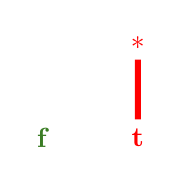
\begin{tikzpicture}[scale=0.4]
			\node (A) at (0,0) {\textcolor{OliveGreen}{\textbf{f}}};
			\node (B) at (3,0) {\textcolor{red}{\textbf{t}}};
			\node (C) at (3,3) {\textcolor{red}{$*$}};
			\draw[red, line width=.03in] (B) -- (C);
		\end{tikzpicture} && 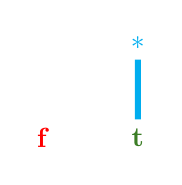
\begin{tikzpicture}[scale=0.4]
		\node (A) at (0,0) {\textcolor{red}{\textbf{f}}};
		\node (B) at (3,0) {\textcolor{OliveGreen}{\textbf{t}}};
		\node (C) at (3,3) {\textcolor{cyan}{$*$}};
		\draw[cyan, line width=.03in] (B) -- (C);
	\end{tikzpicture}
		\arrow["\neg", from=1-1, to=1-3]
	\end{tikzcd}
\caption{$\neg : \Omega \rightarrow \Omega$ in $\mathbb{FF_2}$.}
\end{figure}

Recalling the truth table for $\neg$ in $\mathcal{G}_3$:

	
	\begin{figure}[h]
		\centering
		\begin{tabular}{||c || c ||}  
			\hline
			& $\neg $ \\  
			\hline\hline
			\textcolor{OliveGreen}{\textbf{t}} & \textcolor{red}{\textbf{f}}  \\ 
			\hline
			\textcolor{cyan}{$*$} & \textcolor{red}{\textbf{f}} \\
			\hline
			\textcolor{red}{\textbf{f}} & \textcolor{OliveGreen}{\textbf{t}}  \\
			\hline
		\end{tabular}
		\caption{$\neg$ in $\mathcal{G}_3$.}
	\end{figure}

Looking \emph{from outside} at the $\neg$ arrow for \emph{bushes}, one finds that the nodes \textcolor{OliveGreen}{t} and \textcolor{cyan}{$*$} are mapped to \textcolor{red}{f} and that \textcolor{red}{f} is mapped to \textcolor{OliveGreen}{t}.
\newline
This is precisely the truth function for $\neg$ in $\mathcal{G}_3$. 
\newline
Note that $\neg$ is a unary operator and all one had to do was to look at the nodes in order to \emph{visualize} externally the corresponding truth-table. For binary connectives one needs to look at the product object $\Omega \times \Omega$ and its projections $\pi_1, \pi_2$ and label the nodes appropriately: 
\begin{figure}[h]
	
	\centering
		\begin{tikzcd}
			& 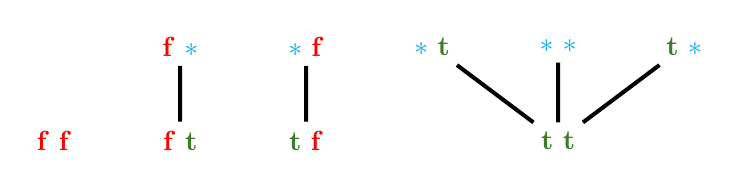
\begin{tikzpicture}[scale=0.4]
				\node (A) at (0,0) {\textcolor{red}{\textbf{f}} \textcolor{red}{\textbf{f}}};
				
				\node (B) at (4,0) {\textcolor{red}{\textbf{f}} \textcolor{OliveGreen}{\textbf{t}}};
				\node (C) at (4,3) {\textcolor{red}{\textbf{f}} \textcolor{cyan}{\textbf{$*$}}};
				
				\node (D) at (8,0) {\textcolor{OliveGreen}{\textbf{t}} \textcolor{red}{\textbf{f}}};
				\node (E) at (8,3) {\textcolor{cyan}{\textbf{$*$}} \textcolor{red}{\textbf{f}}};
				
				\node (F) at (16,0) {\textcolor{OliveGreen}{\textbf{t}} \textcolor{OliveGreen}{\textbf{t}}};
					\node (G) at (12,3) {\textcolor{cyan}{$*$} \textcolor{OliveGreen}{\textbf{t}}};
					\node (H) at (16,3) {\textcolor{cyan}{$*$} \textcolor{cyan}{$*$}};
					\node (I) at (20,3) {\textcolor{OliveGreen}{\textbf{t}} \textcolor{cyan}{$*$}};
				\draw[line width=.02in] (B) -- (C);
				\draw[line width=.02in] (D) -- (E);
				\draw[line width=.02in] (F) -- (G);
				\draw[line width=.02in] (F) -- (H);
				\draw[line width=.02in] (F) -- (I);	
			\end{tikzpicture}
			 \\
			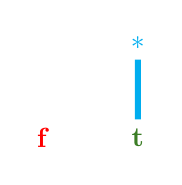
\begin{tikzpicture}[scale=0.4]
				\node (A) at (0,0) {\textcolor{red}{\textbf{f}}};
				\node (B) at (3,0) {\textcolor{OliveGreen}{\textbf{t}}};
				\node (C) at (3,3) {\textcolor{cyan}{$*$}};
				\draw[cyan, line width=.03in] (B) -- (C);
			\end{tikzpicture} && 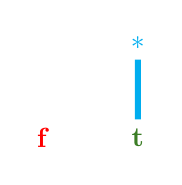
\begin{tikzpicture}[scale=0.4]
			\node (A) at (0,0) {\textcolor{red}{\textbf{f}}};
			\node (B) at (3,0) {\textcolor{OliveGreen}{\textbf{t}}};
			\node (C) at (3,3) {\textcolor{cyan}{$*$}};
			\draw[cyan, line width=.03in] (B) -- (C);
		\end{tikzpicture}
			\arrow["{\pi_1}",dotted, two heads, from=1-2, to=2-1]
			\arrow["{\pi_2}"',dotted, two heads, from=1-2, to=2-3]
		\end{tikzcd}\
		\caption{$\Omega \times \Omega$ and the projections $\pi_1, \pi_2$ to $\Omega$. \newline The nodes of the product are labeled
		in the format $l r$ in which $l$ and $r$ specify the first and second projections respectively:}
\end{figure}

\newpage

Keeping this representation in mind, the same phenomenon we observed for the truth-arrow $\neg$ occurs now for the other connectives.\newline

In other words, we re-discover the truth functions for $\mathcal{G}_3$:
	
	
	\begin{figure}[h]
	\centering
	\begin{subfigure}[h]{0.4\textwidth}
		\begin{tikzcd}
			
\begin{tikzpicture}[scale=0.4]
				\node (A) at (0,0) {\textcolor{red}{$\bigcdot$}};
				\node (B) at (2,0) {\textcolor{red}{$\bigcdot$}};
				\node (C) at (2,3) {\textcolor{red}{$\bigcdot$}};
				\node (D) at (4,0) {\textcolor{red}{$\bigcdot$}};
				\node (E) at (4,3) {\textcolor{red}{$\bigcdot$}};
				\node (F) at (8,0) {\textcolor{OliveGreen}{$\bigcdot$}};
				\node (G) at (6,3) {\textcolor{cyan}{$\bigcdot$}};
				\node (H) at (8,3) {\textcolor{cyan}{$\bigcdot$}};
				\node (I) at (10,3) {\textcolor{cyan}{$\bigcdot$}};
				\draw[red, line width=.03in] (B) -- (C);
				\draw[red, line width=.03in] (D) -- (E);
				\draw[cyan, line width=.03in] (F) -- (G);
				\draw[cyan, line width=.03in] (F) -- (H);
				\draw[cyan, line width=.03in] (F) -- (I);	
			\end{tikzpicture} && 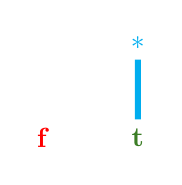
\begin{tikzpicture}[scale=0.4]
				\node (A) at (0,0) {\textcolor{red}{\textbf{f}}};
				\node (B) at (3,0) {\textcolor{OliveGreen}{\textbf{t}}};
				\node (C) at (3,3) {\textcolor{cyan}{$*$}};
				\draw[cyan, line width=.03in] (B) -- (C);
			\end{tikzpicture}
			\arrow["\land", from=1-1, to=1-3]
		\end{tikzcd}
		\caption{$\land : \Omega \times \Omega \rightarrow \Omega$ in $\mathbb{FF_2}$.}
	\end{subfigure}
	\hfill
	\centering
	\begin{subfigure}[h]{0.2\textwidth}
	\begin{tabular}{||c || c | c | c ||}  
		\hline
		$ \land $ & \textcolor{OliveGreen}{\textbf{t}} & \textcolor{cyan}{$*$} & \textcolor{red}{\textbf{f}} \\  
		\hline\hline
		\textcolor{OliveGreen}{\textbf{t}} & \textcolor{OliveGreen}{\textbf{t}} & \textcolor{cyan}{$*$} & \textcolor{red}{\textbf{f}}  \\ 
		\hline
		\textcolor{cyan}{$*$} & \textcolor{cyan}{$*$} & \textcolor{cyan}{$*$} & \textcolor{red}{\textbf{f}} \\
		\hline
		\textcolor{red}{\textbf{f}} & \textcolor{red}{\textbf{f}} & \textcolor{red}{\textbf{f}} & \textcolor{red}{\textbf{f}}  \\
		\hline
	\end{tabular}
	\caption{$\land$ in $\mathcal{G}_3$.}
	\end{subfigure}
	
\end{figure}

	\begin{figure}[h]
	\centering
	\begin{subfigure}[h]{0.4\textwidth}
		\begin{tikzcd}
			
\begin{tikzpicture}[scale=0.4]
			\node (A) at (0,0) {\textcolor{red}{$\bigcdot$}};
			\node (B) at (2,0) {\textcolor{OliveGreen}{$\bigcdot$}};
			\node (C) at (2,3) {\textcolor{cyan}{$\bigcdot$}};
			\node (D) at (4,0) {\textcolor{OliveGreen}{$\bigcdot$}};
			\node (E) at (4,3) {\textcolor{cyan}{$\bigcdot$}};
			\node (F) at (8,0) {\textcolor{OliveGreen}{$\bigcdot$}};
			\node (G) at (6,3) {\textcolor{OliveGreen}{$\bigcdot$}};
			\node (H) at (8,3) {\textcolor{cyan}{$\bigcdot$}};
			\node (I) at (10,3) {\textcolor{OliveGreen}{$\bigcdot$}};
			\draw[cyan, line width=.03in] (B) -- (C);
			\draw[cyan, line width=.03in] (D) -- (E);
			\draw[OliveGreen, line width=.03in] (F) -- (G);
			\draw[cyan, line width=.03in] (F) -- (H);
			\draw[OliveGreen, line width=.03in] (F) -- (I);	
		\end{tikzpicture} &&  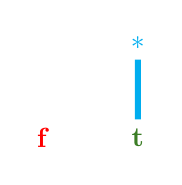
\begin{tikzpicture}[scale=0.4]
		\node (A) at (0,0) {\textcolor{red}{\textbf{f}}};
		\node (B) at (3,0) {\textcolor{OliveGreen}{\textbf{t}}};
		\node (C) at (3,3) {\textcolor{cyan}{$*$}};
		\draw[cyan, line width=.03in] (B) -- (C);
		\end{tikzpicture}
		\arrow["\lor", from=1-1, to=1-3]
		\end{tikzcd}
		\caption{$\lor : \Omega \times \Omega \rightarrow \Omega$ in $\mathbb{FF_2}$.}
	\end{subfigure}
	\hfill
	\centering
	\begin{subfigure}[h]{0.2\textwidth}
		\begin{tabular}{||c || c | c | c ||}  
			\hline
			$ \lor $ & \textcolor{OliveGreen}{\textbf{t}} & \textcolor{cyan}{$*$} & \textcolor{red}{\textbf{f}} \\  
			\hline\hline
			\textcolor{OliveGreen}{\textbf{t}} & \textcolor{OliveGreen}{\textbf{t}} & \textcolor{OliveGreen}{\textbf{t}} & \textcolor{OliveGreen}{\textbf{t}}  \\ 
			\hline
			\textcolor{cyan}{$*$} & \textcolor{OliveGreen}{\textbf{t}} & \textcolor{cyan}{$*$} & \textcolor{cyan}{$*$} \\
			\hline
			\textcolor{red}{\textbf{f}} & \textcolor{OliveGreen}{\textbf{t}} & \textcolor{cyan}{$*$} & \textcolor{red}{\textbf{f}}  \\
			\hline
		\end{tabular}
		\caption{$\lor$ in $\mathcal{G}_3$.}
	\end{subfigure}
	
\end{figure}

	\begin{figure}[h]
	\centering
	\begin{subfigure}[h]{0.4\textwidth}
		\begin{tikzcd}
		
\begin{tikzpicture}[scale=0.4]
			\node (A) at (0,0) {\textcolor{OliveGreen}{$\bigcdot$}};
			\node (B) at (2,0) {\textcolor{OliveGreen}{$\bigcdot$}};
			\node (C) at (2,3) {\textcolor{OliveGreen}{$\bigcdot$}};
			\node (D) at (4,0) {\textcolor{red}{$\bigcdot$}};
			\node (E) at (4,3) {\textcolor{red}{$\bigcdot$}};
			\node (F) at (8,0) {\textcolor{OliveGreen}{$\bigcdot$}};
			\node (G) at (6,3) {\textcolor{OliveGreen}{$\bigcdot$}};
			\node (H) at (8,3) {\textcolor{OliveGreen}{$\bigcdot$}};
			\node (I) at (10,3) {\textcolor{cyan}{$\bigcdot$}};
			\draw[OliveGreen, line width=.03in] (B) -- (C);
			\draw[red, line width=.03in] (D) -- (E);
			\draw[OliveGreen, line width=.03in] (F) -- (G);
			\draw[OliveGreen, line width=.03in] (F) -- (H);
			\draw[cyan, line width=.03in] (F) -- (I);	
		\end{tikzpicture} &&  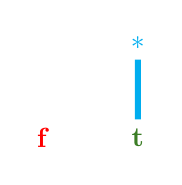
\begin{tikzpicture}[scale=0.4]
				\node (A) at (0,0) {\textcolor{red}{\textbf{f}}};
				\node (B) at (3,0) {\textcolor{OliveGreen}{\textbf{t}}};
				\node (C) at (3,3) {\textcolor{cyan}{$*$}};
				\draw[cyan, line width=.03in] (B) -- (C);
			\end{tikzpicture}
			\arrow["\Rightarrow", from=1-1, to=1-3]
		\end{tikzcd}
		\caption{$\Rightarrow : \Omega \times \Omega \rightarrow \Omega$ in $\mathbb{FF_2}$.}
	\end{subfigure}
	\hfill
	\centering
	\begin{subfigure}[h]{0.2\textwidth}
			\begin{tabular}{||c || c | c | c ||}  
			\hline
			$ \Rightarrow $ & \textcolor{OliveGreen}{\textbf{t}} & \textcolor{SkyBlue}{$*$} & \textcolor{red}{\textbf{f}} \\  
			\hline\hline
			\textcolor{OliveGreen}{\textbf{t}} & \textcolor{OliveGreen}{\textbf{t}} & \textcolor{SkyBlue}{$*$} & \textcolor{red}{\textbf{f}}  \\ 
			\hline
			\textcolor{SkyBlue}{$*$} & \textcolor{OliveGreen}{\textbf{t}} & \textcolor{OliveGreen}{\textbf{t}} & \textcolor{red}{\textbf{f}} \\
			\hline
			\textcolor{red}{\textbf{f}} & \textcolor{OliveGreen}{\textbf{t}} & \textcolor{OliveGreen}{\textbf{t}} & \textcolor{OliveGreen}{\textbf{t}}  \\
			\hline
		\end{tabular}
		\caption{$\Rightarrow$ in $\mathcal{G}_3$.}
	\end{subfigure}
	
\end{figure}

\newpage

\emph{From the inside} however we just defined truth values for  $\mathbb{FF_2}$ as elements of the hom-set $\mathbb{FF_2}(\textbf{1},\Omega) = \{ \top, \bot\}$ i.e., the set containing the arrow $\top$ for which $\bullet \mapsto \textcolor{OliveGreen}{\textbf{t}}$ and $\bot$ for which $\bullet \mapsto \textcolor{red}{\textbf{f}}$.\newline 
Having just two truth-values, the topos $\mathbb{FF_2}$ of \emph{bushes} is called \emph{bivalent}. \newline 
The third node which we labeled \textcolor{cyan}{$*$} and which externally seems to correspond to the same-name truth-value \textcolor{cyan}{$*$} \emph{not-false} in $\mathcal{G}_3$ cannot be a truth-value of the form $\textbf{1} \rightarrow \Omega$ since \textbf{1} as an open map can only be mapped to a root so either to \textcolor{red}{\textbf{f}} or \textcolor{OliveGreen}{\textbf{t}}.\newline
Informally we could say:
\begin{remark}
	 $\mathbb{FF_2}$/\emph{bushes} is \emph{internally} bivalent while \emph{from the outside} $\Omega$ has three elements.
\end{remark}
In other words:
\begin{remark}
	On the propositional level, the \emph{internal} logic of $\mathbb{FF_2}$/\emph{bushes} is classical whilst the \emph{external} logic is that of $\mathcal{G}_3$.
\end{remark}


What does it mean if the topos behaves \emph{classically} on the \emph{inside} and \emph{non-classically} on the \emph{outside}? 
\newpage

To clarify this situation,
let's take a look at what happens with \emph{double negation}. Recall that in classical logic $\alpha$ \emph{is equivalent to} $\neg \neg \alpha$ so we would expect in the language of topoi for the following to hold: $\neg \circ \neg = id_\Omega$.


\begin{figure}[h]
	\centering
	\begin{tikzcd}
		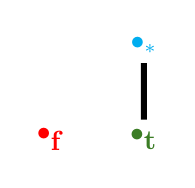
\begin{tikzpicture}[scale=0.4]
			\node (A) at (0,0) {\textcolor{red}{$\bullet_{\textbf{f}}$}};
		\node (B) at (3,0) {\textcolor{OliveGreen}{$\bullet_{\textbf{t}}$}};
		\node (C) at (3,3) {\textcolor{cyan}{$\bullet_{*}$}};
		\draw[line width=.03in] (B) -- (C);
		\end{tikzpicture} & 	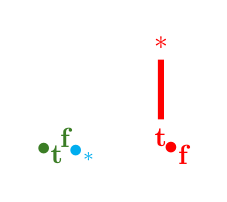
\begin{tikzpicture}[scale=0.4]
		\node (A) at (0,0) {\textcolor{OliveGreen}{\textbf{f}}};
		\node (a) at (-0.5,-0.5) {\textcolor{OliveGreen}{$\bullet_{\textbf{t}}$}};
		\node (a') at (0.5,-0.5) {\textcolor{cyan}{$\bullet_{*}$}};
		\node (b) at (3.5,-0.5) {\textcolor{red}{$\bullet_{\textbf{f}}$}};
		\node (B) at (3,0) {\textcolor{red}{\textbf{t}}};
		\node (C) at (3,3) {\textcolor{red}{$*$}};
		\draw[red, line width=.03in] (B) -- (C);
		\end{tikzpicture} \\
		& 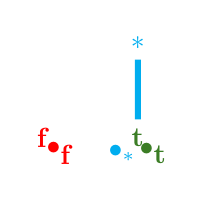
\begin{tikzpicture}[scale=0.4]
			\node (A) at (0,0) {\textcolor{red}{\textbf{f}}};
			\node (a) at (3.5,-0.5) {\textcolor{OliveGreen}{$\bullet_{\textbf{t}}$}};
			\node (a') at (2.5,-0.5) {\textcolor{cyan}{$\bullet_{*}$}};
			\node (b) at (0.5,-0.5) {\textcolor{red}{$\bullet_{\textbf{f}}$}};
			\node (B) at (3,0) {\textcolor{OliveGreen}{\textbf{t}}};
			\node (C) at (3,3) {\textcolor{cyan}{$*$}};
			\draw[cyan, line width=.03in] (B) -- (C);
		\end{tikzpicture}
		\arrow["\neg", from=1-2, to=2-2]
		\arrow["\neg", from=1-1, to=1-2]
		\arrow["{id_\Omega}"', from=1-1, to=2-2]
	\end{tikzcd}
	\caption{$\neg \circ \neg \neq id_\Omega$ in $\mathbb{FF_2}$. \newline Here we displayed the images of the nodes of $\Omega$ in the top left corner as labeled bullets. }
\end{figure}
	
	This is clearly not the case for our topos.
	\newline
	Note that while the \emph{classical} nodes \textcolor{OliveGreen}{$\bullet_{\textbf{t}}$} $\mapsto \textcolor{OliveGreen}{\textbf{t}}$, \textcolor{red}{$\bullet_{\textbf{f}}$} $\mapsto \textcolor{red}{\textbf{f}}$ are fixed by $\neg \circ \neg$, the \emph{non-classical} node \textcolor{cyan}{$\bullet_{*}$}$\mapsto \textcolor{OliveGreen}{\textbf{t}}$ is not.\footnote{this corresponds to the fact in $\mathcal{G}_3$ that the negation of $*$ i.e., \emph{not-false} is \emph{false}. }\newline
	
	Another approach is to consider the \emph{Algebra of sub-objects}. \newline
	When in a topos the algebra of sub-objects for an arbitrary object, which we have seen is a Heyting Algebra, is also a Boolean Algebra:
	
	\begin{definition}[Boolean topos]
		A topos $\mathcal{E}$ is \emph{Boolean} if for every object $\textbf{d}$, $(Sub(\textbf{d}), \sqsubseteq)$ is a Boolean Algebra.
	\end{definition} 
	
	\begin{ex}[Sets]
		The prototypical Boolean topos is unsurprisingly $\mathbb{Set}$ where for every set $D$ it is the case that  $(Sub(\textbf{D}), \sqsubseteq) \cong (\mathcal{P}(D), \subseteq)$ which is the \emph{power-set} Boolean Algebra.
	\end{ex}
	
	We can use the following results from \cite{goldblatt} and \cite{lambekscott}:
	
	\begin{lem}
		For any topos $\mathcal{E}$, $\mathcal{E}$ is Boolean iff $(Sub(\Omega),\sqsubseteq)$ is a Boolean Algebra. 
	\end{lem}

	\begin{prop}
		A topos $\mathcal{E}$ is Boolean iff $\textbf{1} \xrightarrow{\top} \Omega \xleftarrow{\bot} \textbf{1}$ is a Co-product diagram.
	\end{prop}
	This would entail $\Omega \cong \textbf{1} + \textbf{1}$ and $\neg\circ\neg = id_\Omega$ which are both false for \emph{bushes}.\newline 

We also know that $\Omega = Spec(\mathcal{F}_1)$ i.e., the prime spectrum of the free Gödel Algebra on one generator $\mathcal{F}_1$. $Sub(Spec(\mathcal{F}_1))$ are in this case the sub-forests of the prime spectrum of $\mathcal{F}_1$ and by duality we have shown that  $Sub(Spec(\mathcal{F}_1)) \cong \mathcal{F}_1$. 
\newline
	$\mathcal{F}_1$ is not a Boolean Algebra ($(x \lor \neg x) \neq 1$) and so, summing up: 
	
	\begin{thm}[propositional logic of $\mathbb{FF_2}$]
		${}$ \newline
		The topos of \emph{bushes} $\mathbb{FF_2}$ is bivalent and non-Boolean.
	\end{thm}
	
	By a direct application of (\ref{bivalence}) we obtain:
	\begin{cor}
		\begin{equation*}
			\forall \alpha \in \textbf{Form} : \;\vdash_{CPL} \alpha \;\text{ iff }\; \mathbb{FF_2} \models \alpha.
		\end{equation*}
	\end{cor}

\newpage	
\subsection{A few Topoi Examples}
\label{examples}
	
	To better understand why for topoi \emph{bivalent} and \emph{Boolean} are, in a sense, independent attributes, consider the following examples:\newline
	(We omit in both cases the construction of exponential objects and focus on their sub-object classifier and truth-arrows).
	
	\begin{ex}[Pair of Sets]
		The topos $ \mathbb{Set}^2 $ of \emph{Pairs of Sets} has as objects all set pairs $\langle A,B \rangle$ and arrows pairs of set functions $\langle f, g \rangle :  \langle A,B \rangle \rightarrow \langle C,D \rangle$ with $f: A \rightarrow C$ and $g: B \rightarrow D$.\newline
		
		One can verify that the sub-object classifier $\Omega$ for $ \mathbb{Set}^2 $ is none-other than 
		$\langle \textbf{2}, \textbf{2} \rangle $ with the \emph{true} arrow given by $\langle \top,\top \rangle : \langle \{0\},\{0\} \rangle \rightarrow \langle \textbf{2}, \textbf{2} \rangle $.\newline
		As such, the \emph{truth values} are precisely the four elements $\{ \langle \bot,\bot \rangle, \langle \bot,\top \rangle, \langle \top,\bot \rangle, \langle \top,\top \rangle \}$. 
	\end{ex} 
	So:
	\begin{remark}
		$ \mathbb{Set}^2 $ fails to be bivalent. It is however a Boolean topos as the sub-objects of $\Omega$ form a power-set Boolean Algebra.\footnote{see \cite{goldblatt} for details.}  
	\end{remark}
	
	\begin{ex}[Functions between sets]
		The \emph{functor category} $\mathbb{Set}^{0 \rightarrow 1}$ of \emph{functions between sets}, with objects the functors $F :\mathbb{2} \rightarrow \mathbb{Set}$ from the poset category $\mathbf{2}:=\{0 \xrightarrow{\leq_0}$ 1\}\footnote{$\mathbf{2}$ has only objects 0 and 1 and the only non-identity arrow 01 from 0 to 1.} to $\mathbb{Set}$ and arrows the natural transformations $\tau : F \Rightarrow G$ between these functors, is a topos.
		 \newline
		We use the notation $F_i, G_j$ for $F(i),G(j)$. Also $f$ replaces $F(\leq_0)$ and $g$ replaces $G(\leq_0)$.\newline
		
		An arrow $\tau$ from the objects $F$ and $G$ is realized in $\mathbb{Set}$ as a commutative diagram:
		
		\begin{figure}[h]
			\centering
			\begin{tikzcd}
				0 && {F_0} & {G_0} \\
				1 && {F_1} & {G_1}
				\arrow[from=1-1, to=2-1]
				\arrow["{\tau_0}"', from=1-3, to=1-4]
				\arrow["f", from=1-3, to=2-3]
				\arrow["{\tau_1}"', from=2-3, to=2-4]
				\arrow["g", from=1-4, to=2-4]
			\end{tikzcd}\
			\caption{The poset category $\mathbb{2}$ (left) and the commutative diagram in $\mathbb{Set}$ (right).}
		\end{figure}  
		
		The terminal object \textbf{1}, one can verify, is the identity function $\{0\} \xrightarrow{id} \{0\}$ on the singleton set $\{0\}$. \newline
		The sub-object $\mu : F \Rightarrow G$ is realized again as a commutative diagram and we will assume without loss of generality  that the components $\mu_0, \mu_1$ (which are injective functions in $\mathbb{Set}$) be set-inclusions $F_0 \subseteq G_0, F_1 \subseteq G_1$  so that $f$ will in fact be the restriction of $g$ to $F_0$. 
		\begin{figure}[h]
			\centering
			\begin{tikzcd}
				{F_0} & {G_0} \\
				{F_1} & {G_1}
				\arrow["{\mu_0}", tail, from=1-1, to=1-2]
				\arrow["{f = g \restriction F_0}"', from=1-1, to=2-1]
				\arrow["{\mu_1}"', tail, from=2-1, to=2-2]
				\arrow["g", from=1-2, to=2-2]
			\end{tikzcd}
			\caption{The sub-object $\mu : F \Rightarrow G$.}
		\end{figure}
		\newline
		Note that an element $x \in G_0$ can be \emph{classified} in three ways:
		\begin{enumerate}[label=(\roman*)]
			\item $x \in F_0$.
			\item $x \notin F_0$ but $g(x) \in F_1$.
			\item $x \notin F_0$ and $g(x) \notin F_1$.
		\end{enumerate}
		 For this purpose, we introduce the set $\{0,\frac{1}{2},1\}$ and define $\psi : F_0 \rightarrow \{0,\frac{1}{2},1\}$ by:
		 \begin{equation*}
		 	\psi(x) =
		 	\begin{cases}
		 		1 & \text{if (i) holds}\\
		 		\frac{1}{2} & \text{if (ii) holds}\\
		 		0 & \text{if (iii) holds}
		 	\end{cases}       
		 \end{equation*}  
		  
		  \begin{figure}[h]
		  	\centering
		  	
		  	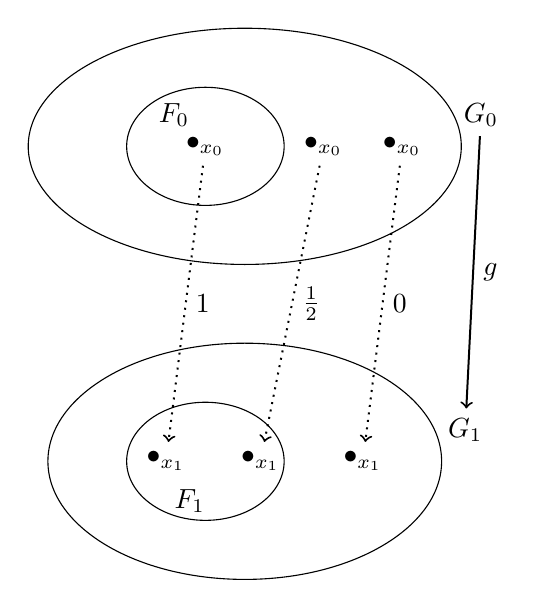
\begin{tikzpicture}
		  		\node (a) at (-0.4,0.4) {$F_0$};
		  		\node (b) at (3.5,0.4) {$G_0$};
		  		\node (A0) at (0,0) {$\bullet_{x_0}$};
		  		\node (B0) at (1.5,0) {$\bullet_{x_0}$};
		  		\node (C0) at (2.5,0) {$\bullet_{x_0}$};
		  		\draw (0.5,0) ellipse (2.75 and 1.5);
		  		\draw (0,0) ellipse (1 and 0.75);
		  		
		  		\draw (0.5,-4) ellipse (2.5 and 1.5);
		  		\draw (0,-4) ellipse (1 and 0.75);
		  		\node (A1) at (-0.5,-4) {$\bullet_{x_1}$};
		  		\node (B1) at (0.7,-4) {$\bullet_{x_1}$};
		  		\node (C1) at (2,-4) {$\bullet_{x_1}$};
		  		\node (c) at (-0.2,-4.5) {$F_1$};
		  		\node (d) at (3.3,-3.6) {$G_1$};
		  		
		  		\draw[->, dotted, line width=.01in] (A0) -- node[anchor=west] {$1$} (A1);
		  		\draw[->, dotted, line width=.01in] (B0) -- node[anchor=west] {$\frac{1}{2}$} (B1);
		  		\draw[->, dotted, line width=.01in] (C0) -- node[anchor=west] {$0$} (C1);
		  		\draw[->, line width=.01in] (b) -- node[anchor=west] {$g$} (d);
		  	\end{tikzpicture}
		  	\caption{The sub-object $F \xRightarrow{\mu} G$ and the function $\psi$.}
		  \end{figure}
		  
		  This suggests that: \newline
		   $\Omega(0) := \{0,\frac{1}{2},1\}$ and $\Omega(1) := \{0,1\}$ with $\Omega(\leq_0):= t: 0 \mapsto 0, \frac{1}{2} \mapsto 1, 1 \mapsto 1$. 
\newpage
		  The sub-object classifier is thus given by $\top : \textbf{1} \Rightarrow \Omega$:
		  
		  \begin{figure}[h]
		  	\centering
			\begin{tikzcd}
				{\{0\}} && {\{0,\frac{1}{2},1\}} \\
				& {{}} \\
				{\{0\}} && {\{0,1\}}
				\arrow[draw=none, from=1-1, to=2-2]
				\arrow["{t'}", from=1-1, to=1-3]
				\arrow["id"', from=1-1, to=3-1]
				\arrow["true"', from=3-1, to=3-3]
				\arrow["t", from=1-3, to=3-3]
			\end{tikzcd}
		  	\caption{$true: 0 \mapsto 1$, $t': 0 \mapsto 1$, $t:  0 \mapsto 0, \frac{1}{2} \mapsto 1, 1 \mapsto 1$.}
		  \end{figure}
		  
		  We have in addition to $\top$ other two truth-arrows $*,  \bot : \textbf{1} \Rightarrow \Omega$:
		  	\begin{figure}[h]
		  		\centering
		  			\begin{tikzcd}
		  			{\{0\}} && {\{0,\frac{1}{2},1\}} \\
		  			& {{}} \\
		  			{\{0\}} && {\{0,1\}}
		  			\arrow[draw=none, from=1-1, to=2-2]
		  			\arrow["{*'}", from=1-1, to=1-3]
		  			\arrow["id"', from=1-1, to=3-1]
		  			\arrow["true"', from=3-1, to=3-3]
		  			\arrow["t", from=1-3, to=3-3]
		  		\end{tikzcd}
		  		\caption{$* : \textbf{1} \Rightarrow \Omega$ with
		  			$true: 0 \mapsto 1$, $*': 0 \mapsto \frac{1}{2}$.}
		  	\end{figure}
		  
		  	\begin{figure}[h]
		  		\centering
		  		\begin{tikzcd}
		  			{\{0\}} && {\{0,\frac{1}{2},1\}} \\
		  			& {{}} \\
		  			{\{0\}} && {\{0,1\}}
		  			\arrow[draw=none, from=1-1, to=2-2]
		  			\arrow["{f'}", from=1-1, to=1-3]
		  			\arrow["id"', from=1-1, to=3-1]
		  			\arrow["false"', from=3-1, to=3-3]
		  			\arrow["t", from=1-3, to=3-3]
		  		\end{tikzcd}
		  		\caption{$\bot : \textbf{1} \Rightarrow \Omega$ with
		  			$false: 0 \mapsto 0$, $f': 0 \mapsto 0$.}
		  	\end{figure}
	
		  \newpage
		  The characteristic diagram is now a cube instead of the usual square:
		  
		  \begin{figure}[h]
		  	\centering
		  	\begin{tikzcd}
		  	{F_0} && {G_0} \\
		  	& {F_1} && {G_1} \\
		  	{\{0\}} && {\{0,\frac{1}{2},1\}} \\
		  	& {\{0\}} && {\{0,1\}}
		  	\arrow["true"', from=4-2, to=4-4]
		  	\arrow["id"', from=3-1, to=4-2]
		  	\arrow["{t'}"'{pos=0.6}, from=3-1, to=3-3]
		  	\arrow["t", from=3-3, to=4-4]
		  	\arrow["{\tau_0}", tail, from=1-1, to=1-3]
		  	\arrow[""{name=0, anchor=center, inner sep=0}, "f"', from=1-1, to=2-2]
		  	\arrow["g"', from=1-3, to=2-4]
		  	\arrow["{\tau_1}", tail, from=2-2, to=2-4]
		  	\arrow["{\chi_{F_1}}", from=2-4, to=4-4]
		  	\arrow[dashed, from=2-2, to=4-2]
		  	\arrow[dashed, from=1-1, to=3-1]
		  	\arrow["\psi"'{pos=0.6}, dotted, from=1-3, to=3-3]
		  		\arrow[draw=none, from=2-2, to=3-3]
		  			\arrow[ from=2-2, to=3-3, phantom, "\scalebox{1.5}{$\lrcorner$}",  very near start, color=black]
		  		\arrow[draw=none, from=1-1, to=0]
		  			\arrow[ from=1-1, to=0, phantom, "\scalebox{1.5}{$\lrcorner$}",  very near start, color=black]
		  	\end{tikzcd}
		  	\caption{The front and back faces of the cube are each pull-backs in $\mathbb{Set}$.}
		  \end{figure}
		  	  	  
	\end{ex}
	
The following holds: \footnote{to prove that  $\mathbb{Set}^{0 \rightarrow 1}$ is not a Boolean topos requires some further considerations that will be made later on.}

	\begin{remark}
		 $\mathbb{Set}^{0 \rightarrow 1}$ is neither bivalent (it has three truth-arrows) nor Boolean.
	\end{remark}

\newpage
A generalized version of $\mathbb{Set}^{0 \rightarrow 1}$, which will prove rather important later on, is that of the functor category of \emph{sets through time}:

\begin{ex}[Sets through time]
	Let $\mathbf{\omega}:=(\omega, \leq) $ be the poset category of natural numbers with their standard ordering $0 \xrightarrow{\leq_0} 1 \xrightarrow{\leq_1} 2 \xrightarrow{\leq_2}...$ which will be our so-called \emph{moments in time}. \newline 
	$\mathbb{Set}^\mathbf{\omega}$, a.k.a. the category of \emph{sets through time} has objects \emph{sequences} of sets and arrows \emph{commutative diagrams} between them:
	
	\begin{figure}[h]
		\centering
	\begin{tikzcd}
		{F:} & {F_0} & {F_1} & {F_2} & {...} & {F_m} & {F_{m+1}} & {...} \\
		{G:} & {G_0} & {G_1} & {G_2} & {...} & {G_m} & {G_{m+1}} & {...}
		\arrow["{F_{12}}"', from=1-3, to=1-4]
		\arrow[from=1-4, to=1-5]
		\arrow[from=1-5, to=1-6]
		\arrow["{F_{m\;m+1}}", from=1-6, to=1-7]
		\arrow["{F_{01}}"', from=1-2, to=1-3]
		\arrow[from=1-7, to=1-8]
		\arrow[from=2-2, to=2-3]
		\arrow["{G_{12}}"', from=2-3, to=2-4]
		\arrow[from=2-4, to=2-5]
		\arrow[from=2-5, to=2-6]
		\arrow["{G_{m\;m+1}}"', from=2-6, to=2-7]
		\arrow[from=2-7, to=2-8]
		\arrow["{\tau_{m+1}}", dashed, from=1-7, to=2-7]
		\arrow["{\tau_m}", dashed, from=1-6, to=2-6]
		\arrow["{\tau_2}", dashed, from=1-4, to=2-4]
		\arrow["{\tau_1}", dashed, from=1-3, to=2-3]
		\arrow["{\tau_0}", dashed, from=1-2, to=2-2]
		\arrow["\tau", squiggly, from=1-1, to=2-1]
	\end{tikzcd}
		\caption{$\tau : F \Rightarrow G$.}
	\end{figure}  
	
	 It is worth pausing to give an intuition due to \emph{John C. Baez} for the notion of \emph{sets through time}:
	
	\begin{remark}
		Imagine a set of theorems proven by an infallible mathematician at various times $0,1,2.. \in \omega$.\newline
		As time passes, in steps from $0$ to $1$ and from $1$ to $2$ and so on, This set can get new elements as the mathematician produces new theorems.\newline
		Also, two distinct theorems can \emph{merge} into one if an equivalence is found between them. \newline
		However, we can never remove an element from the set as once a theorem has been proven it remains so forever and cannot be dis-proven.  
	\end{remark}
	
	Notice that: 
	Any non-empty up-set $S\subseteq \omega$ has a minimum $m_S$ and so we have:
	\begin{equation*}
		S = [m_S) = \{m_S, m_S +1, m_S +2...\}.
	\end{equation*}
	 i.e., $S$ coincides with the principal up-set generated by its minimum. \newline
	
	Now let us add a symbol for \emph{infinity} to replace the empty-set so that $S=\emptyset$ becomes $S=\{\infty\}$. \newline
	So we work with $\mathbf{\omega}^+ := \mathbf{\omega} \cup \{\infty\}$.\newline
	
	The terminal object, a.k.a. \emph{the infinite telephone pole}  is the constant functor $\textbf{1}$ :
	\begin{gather*}
		\forall m\in \omega : \textbf{1}(m) := \{0\}. \\
		\textbf{1}(\leq_m) := id_{\{0\}}. 
	\end{gather*}
	 
	
	For the sub-object classifier, $\Omega$ and $\top : \textbf{1} \Rightarrow \Omega$ are defined in the following way for each $m \in \mathbf{\omega}$ : \footnote{we make use of the same notation we introduced for the previous example.}
	\begin{gather*}
		m \;\mapsto\; \Omega_m := [m) = \{m,m+1,..,\infty\}. \\
		m \xrightarrow{\leq} n \;\mapsto\;\; [m)  \xrightarrow{\Omega_{m\;n}} [n) \text{ where } 
		\Omega_{m\;n}(p) :=
		\begin{cases}
			n & \text{if } m \leq p \leq n \\
			p & \text{if } n \leq p \\
			\infty & \text{if } p = \infty
		\end{cases}. \\
		 \top_m: \{0\} \rightarrow  [m) \text{ where } \top_m(0) := m.
	\end{gather*} 
	\newpage
	We can display $\Omega$ as:
	
	\begin{figure}[h]
		\centering
	\begin{tikzcd}
		{\Omega_m =} & {\{} & {m,} & {m+1,} & {m+2,} & {...} & \infty & {\}} \\
		{\Omega_{m+1} =} & {\{} & {m+1,} & {m+2,} & {...} & {...} & \infty & {\}} \\
		{\Omega_{m+2} =} & {\{} & {m+2,} & {...} & {...} & {...} & \infty & {\}} \\
		&& {} & {} & {...} & {...} \\
		{\Omega_n =} & {\{} & {n,} & {n+1,} & {...} & {...} & \infty & {\}}
		\arrow["{\Omega_{m \; m+1}}"', from=1-1, to=2-1]
		\arrow[maps to, from=1-3, to=2-3]
		\arrow[maps to, from=1-4, to=2-3]
		\arrow[maps to, from=1-5, to=2-4]
		\arrow["{\Omega_{m+1 \; m+2}}"', from=2-1, to=3-1]
		\arrow[maps to, from=2-3, to=3-3]
		\arrow[maps to, from=2-4, to=3-3]
		\arrow["{\Omega_{m+2 \; n}}"', dotted, from=3-1, to=5-1]
		\arrow[dashed, maps to, from=3-3, to=4-3]
		\arrow[dashed, maps to, from=4-3, to=5-3]
		\arrow[dashed, maps to, from=4-4, to=5-3]
		\arrow[dashed, maps to, from=1-6, to=2-5]
		\arrow[dashed, maps to, from=2-5, to=3-4]
		\arrow[dashed, maps to, from=3-4, to=4-3]
		\arrow[maps to, from=1-7, to=2-7]
		\arrow[maps to, from=2-7, to=3-7]
		\arrow[dashed, maps to, from=3-7, to=5-7]
	\end{tikzcd}
		\caption{$\Omega$ displayed in a few of its components.}
	\end{figure}
	
	\newpage
	The characteristic arrow $\chi_\tau$ of a sub-object $\tau : F \Rightarrow G$ (as before w.l.o.g. we assume $F_m \subseteq G_m$) is given by the so-called \emph{time till truth}:
	\begin{equation*}
		(\chi_\tau)_m(x) := \begin{cases}
			min\{n : n\geq m|\; G_{m\;n}(x) \in F_n \} & \text{ if such $n$ exists. } \\
			\infty & \text{ if } G_{m\;n}(x) \notin F_n \text{ for every } n \geq m. 
		\end{cases}
	\end{equation*} 
	
	This is rendered visually as:
	
	\begin{figure}[h]
		\centering
		
		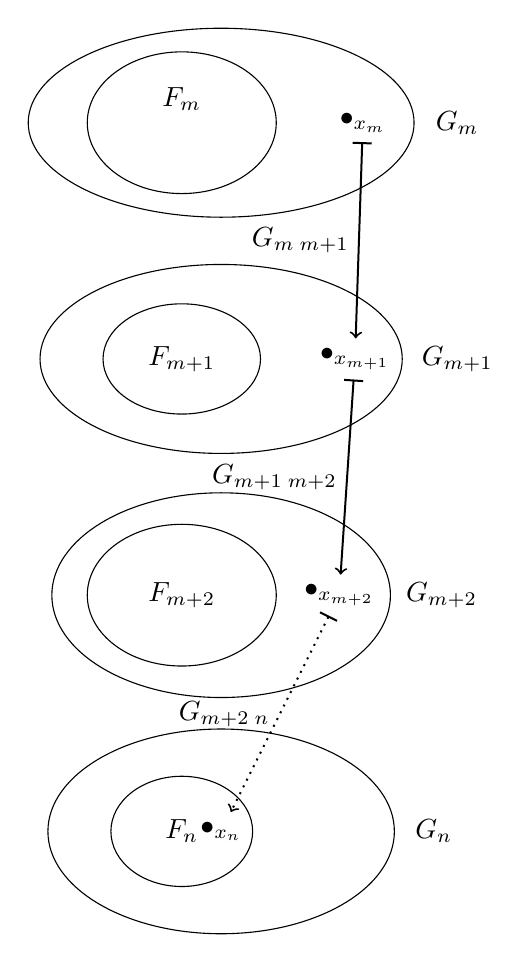
\begin{tikzpicture}
			\node (a) at (0,0.3) {$F_m$};
			\node (b) at (3.5,0) {$G_m$};
			\node (C0) at (2.3,0) {$\bullet_{x_m}$};
			\draw (0.5,0) ellipse (2.45 and 1.2);
			\draw (0,0) ellipse (1.2 and 0.9);
			
			\draw (0.5,-3) ellipse (2.3 and 1.2);
			\draw (0,-3) ellipse (1 and 0.7);
			\node (C1) at (2.2,-3) {$\bullet_{x_{m+1}}$};
			\node (c) at (0,-3) {$F_{m+1}$};
			\node (d) at (3.5,-3) {$G_{m+1}$};
			
			\draw (0.5,-6) ellipse (2.15 and 1.3);
			\draw (0,-6) ellipse (1.2 and 0.9);
			\node (C2) at (2,-6) {$\bullet_{x_{m+2}}$};
			\node (e) at (0,-6) {$F_{m+2}$};
			\node (f) at (3.3,-6) {$G_{m+2}$};
			
			\draw (0.5,-9) ellipse (2.2 and 1.3);
			\draw (0,-9) ellipse (0.9 and 0.7);
			\node (C3) at (0.5,-9) {$\bullet_{x_{n}}$};
			\node (e) at (0,-9) {$F_{n}$};
			\node (f) at (3.2,-9) {$G_{n}$};
			
			\draw[|->, line width=.01in] (C0) -- node[anchor=east] {$G_{m \; m+1}$} (C1);
			\draw[|->, line width=.01in] (C1) -- node[anchor=east] {$G_{m+1 \;m+2}$} (C2);
			\draw[|->, dotted, line width=.01in] (C2) -- node[anchor=east] {$G_{m+2 \;n}$} (C3);
		\end{tikzpicture}
		\caption{Here $(\chi_\tau)_m(x)=n$. \newline
			The sub-object $F \xRightarrow{\tau} G$ is displayed in some of its components $F_m \subseteq G_m$,  $F_{m+1} \subseteq G_{m+1},$ and $F_n \subseteq G_n$  and the transition function $G_{m\;n}$ is shown in its constituents $G_{m\;n}= G_{m\;m+1} G_{m+1\;m+2}G_{m+2 \;n}$.}
	\end{figure}
	
	\newpage
	Notice that we now have a countable infinity of \emph{truth-values} between 
	$\bot : \textbf{1} \Rightarrow \Omega $:
	\begin{gather*}
		\forall m \in \omega :
		(\bot)_m(0) := \{\infty\}. 
	\end{gather*}
	and $\top : \textbf{1} \Rightarrow \Omega$ given by $\{ *_q \}_{q\in \omega}$ where each
	$*_q : \textbf{1} \Rightarrow \Omega$ is given by:
	\begin{gather*}
		\forall m \in \omega :
		(*_q)_m(0) := \begin{cases}
			q & \text{ if }m \leq q. \\
			m & \text{ if }m > q. 
		\end{cases}.
	\end{gather*}
	
	
	
\end{ex}





	\newpage
${}$ \newpage





